\documentclass[aspectratio=169,11pt]{beamer}

\usepackage{amsmath,amssymb,bm}
\usepackage{booktabs}
\usepackage{tikz}
\usepackage{xcolor}
\usetikzlibrary{arrows.meta,positioning,fit}

\definecolor{navy}{HTML}{062B63}
\definecolor{orange}{HTML}{F36F21}
\definecolor{lightblue}{HTML}{EAF2FA}
\definecolor{lightgreen}{HTML}{EAF4E3}
\definecolor{warmgray}{HTML}{F3F4F6}
\definecolor{darkgray}{HTML}{28323C}
\definecolor{muted}{HTML}{66717D}

\setbeamercolor{normal text}{fg=darkgray,bg=white}
\setbeamercolor{structure}{fg=navy}
\setbeamercolor{frametitle}{fg=white,bg=navy}
\setbeamercolor{title}{fg=white}
\setbeamercolor{subtitle}{fg=white}
\setbeamercolor{block title}{fg=white,bg=navy}
\setbeamercolor{block body}{fg=darkgray,bg=lightblue}
\setbeamercolor{alertblock title}{fg=white,bg=orange}
\setbeamercolor{alertblock body}{fg=darkgray,bg=warmgray}
\setbeamercolor{exampleblock title}{fg=white,bg=darkgray}
\setbeamercolor{exampleblock body}{fg=darkgray,bg=lightgreen}

\setbeamertemplate{navigation symbols}{}
\setbeamertemplate{itemize item}{\color{orange}\small$\blacktriangleright$}
\setbeamertemplate{itemize subitem}{\color{navy}\scriptsize$\bullet$}
\setbeamertemplate{enumerate item}{\color{orange}\insertenumlabel.}
\setbeamertemplate{blocks}[rounded][shadow=false]
\setbeamertemplate{frametitle}{%
  \nointerlineskip
  \begin{beamercolorbox}[wd=\paperwidth,ht=0.82cm,dp=0.22cm,leftskip=0.48cm]{frametitle}
    \usebeamerfont{frametitle}\insertframetitle
  \end{beamercolorbox}}
\setbeamertemplate{footline}{%
  \leavevmode%
  \hbox{%
  \begin{beamercolorbox}[wd=.78\paperwidth,ht=2.6ex,dp=1.1ex,leftskip=.45cm]{author in head/foot}%
    \color{muted}\scriptsize Qianhong Zhao \;|\; Human--Robot Co-Manipulation
  \end{beamercolorbox}%
  \begin{beamercolorbox}[wd=.22\paperwidth,ht=2.6ex,dp=1.1ex,rightskip=.45cm plus1fil]{date in head/foot}%
    \color{muted}\scriptsize \insertframenumber/\inserttotalframenumber
  \end{beamercolorbox}}}

\setbeamerfont{title}{size=\fontsize{25}{29},series=\bfseries}
\setbeamerfont{subtitle}{size=\fontsize{14}{18}}
\setbeamerfont{frametitle}{size=\fontsize{15.5}{18},series=\bfseries}
\setbeamerfont{block title}{size=\normalsize,series=\bfseries}
\setbeamerfont{block body}{size=\small}

\newcommand{\key}[1]{\textcolor{orange}{\textbf{#1}}}
\newcommand{\paperout}[1]{%
  \begin{beamercolorbox}[rounded=true,sep=0.55em,wd=\linewidth]{block body}
    \footnotesize\textbf{Expected paper:} #1
  \end{beamercolorbox}}

\title{Generalizable Human Modeling for\\Physical Human--Robot Co-Manipulation}
\subtitle{Connecting multimodal interaction, structured human models,\\and safe robot planning and control}
\author{Qianhong Zhao}
\date{Research Discussion with RISE Lab}

\begin{document}

{\setbeamertemplate{footline}{}
\begin{frame}[plain]
  \begin{tikzpicture}[remember picture,overlay]
    \fill[navy] (current page.south west) rectangle (current page.north east);
    \fill[orange] (current page.north west) rectangle ([xshift=0.22cm]current page.south west);
    \draw[orange,line width=1.2pt] ([xshift=1.0cm,yshift=-2.12cm]current page.north west) -- ([xshift=-1.0cm,yshift=-2.12cm]current page.north east);
  \end{tikzpicture}
  \vspace{0.95cm}
  {\color{white}\fontsize{20.5}{25}\selectfont\bfseries
  Generalizable Human Modeling for\\[0.12cm]
  Physical Human--Robot Co-Manipulation\par}
  \vspace{0.55cm}
  {\color{white}\fontsize{14}{18}\selectfont
  Connecting multimodal interaction, structured human models,\\
  and safe robot planning and control\par}
  \vfill
  {\color{white}\normalsize Qianhong Zhao\par}
  \vspace{0.12cm}
  {\color{white!72}\small Research Discussion with RISE Lab\par}
  \vspace{0.52cm}

  \textcolor{pink}{1. Background color needs to be replaced to some light color. Do not includ too much blue;
  2. The origin line breaks the title. Use another method to underline the title
  }
\end{frame}}

\begin{frame}[shrink=6]{Co-manipulation requires coordination through human uncertainty}
\begin{columns}[T,onlytextwidth]
  \column{0.52\textwidth}
  \begin{block}{Physical co-manipulation}
  A human and a robot physically manipulate a shared object to accomplish a common task safely and efficiently.
  \end{block}
  \vspace{0.15cm}
  \textbf{The robot must simultaneously:}
  \begin{itemize}
    \item infer the human's intent and interaction strategy;
    \item predict responses to robot actions;
    \item coordinate motion and interaction forces;
    \item adapt to individual behavior and strategy changes;
    \item satisfy physical, actuation, and safety constraints.
  \end{itemize}

  \column{0.44\textwidth}
  \begin{alertblock}{Central research question}
  How can the robot model the human well enough to support real-time planning and control? \textcolor{pink}{How to model the human well enough to support real-time planning and control of robot in comipulation tasks? }
  \end{alertblock}
  \vspace{0.25cm}
  \begin{exampleblock}{Desired outcome}
  An explicit human model that is predictive, interactive, uncertainty-aware, and adaptable online.
  \end{exampleblock}
\end{columns}

\textcolor{pink}{1. why explicit human model? if we introduce the complex models for the features of the potential cost functions, how can this model be explicit?
2. current title needs to be modified. the title looks not complete}
\end{frame}

\begin{frame}{Human behavior is structured, adaptive, and bounded-rational}
\begin{columns}[T,onlytextwidth]
\column{0.48\textwidth}
\begin{itemize}
  \item \key{Multimodal}: multiple strategies may be reasonable in the same situation. \textcolor{pink}{ Should multimodal be the  different data types input for the model}
  \item \key{Interactive}: behavior depends on what the robot does.
  \item \key{Bounded-rational}: people may be delayed, inconsistent, or effort-limited.
\end{itemize}
\column{0.48\textwidth}
\begin{itemize}
  \item \key{Adaptive}: people infer the robot's intent and change their behavior.
  \item \key{Person-dependent}: roles, preferences, and control styles differ.
  \item \key{Task-conditioned}: concrete goals change, but some latent concepts transfer.
\end{itemize}
\end{columns}
\vspace{0.35cm}
\begin{block}{Implication}
A useful model must distinguish human intent, interaction style, adaptation, and action uncertainty---without requiring a separate model for every task. 
\end{block}
\end{frame}

\begin{frame}{The shared papers provide complementary foundations}
\small
\begin{columns}[T,onlytextwidth]
\column{0.315\textwidth}
\begin{block}{Diffusion Co-Policy}
\begin{itemize}
  \item Learns multimodal collaborative action sequences \textcolor{pink}{1. looks the input of this paper is "人的输入 a
t
H
	​

：二维力，2D
机器人的输入 a
t
R
	​

：二维力，2D
联合系统输入 a
t
	​

：四维，4D", why you say multimodal.? 2. mention this paper offers the desired test setting for the projects} 
  \item Demonstrates mutual adaptation and role switching
  \item Works with real humans in collaborative carrying
\end{itemize}
\end{block}
\column{0.315\textwidth}
\begin{block}{Bounded-Rational Model}
\begin{itemize}
  \item Models human joint action game-theoretically
  \item Fits behavior better with bounded rationality 
  \item Reveals leadership and adaptation effects
\end{itemize}

\textcolor{pink}{Here needs to mention that this paper convince people that human intention could be modeled through gametheory}
\end{block}
\column{0.315\textwidth}
\begin{block}{PACE / N-PACE}
\begin{itemize}
  \item Infers intent and cost parameters online
  \item Treats the peer as another adapting learner
  \item Connects inference with interaction policies
\end{itemize}
\textcolor{pink}{Here needs to mention that this paper convince people that the comanipulation problem could be solved or solved better based on gametheory and reasonable human inention model}
\end{block}
\end{columns}
\vspace{0.28cm}
\begin{alertblock}{Combined insight}
Learned models provide behavioral flexibility; game-theoretic models provide structure, interpretability, and a connection to control. 
\end{alertblock}
\end{frame}

\begin{frame}{A human-modeling gap remains in physical interaction}
\begin{columns}[T,onlytextwidth]
\column{0.48\textwidth}
\begin{block}{Learned co-policies}
\begin{itemize}
  \item Model the human mostly implicitly
  \item Often require task-specific demonstrations
  \item Do not explicitly represent intent, belief, or preference
  \item Offer limited physical and safety guarantees
\end{itemize}
\end{block}
\column{0.48\textwidth}
\begin{block}{Game / IOC models}
\begin{itemize}
  \item Require predefined cost features
  \item Often assume known intent or learning structures
  \item Struggle with multimodal, history-dependent behavior
  \item May require redesign when the task changes
\end{itemize}
\end{block}
\end{columns}
\vspace{0.25cm}
\begin{alertblock}{Research gap}
Physical co-manipulation needs an explicit but flexible human model that connects motion, force/torque, and task context to robot planning and control.
\end{alertblock}
\end{frame}

\begin{frame}{Predict human responses to candidate robot actions}
\begin{columns}[c,onlytextwidth]
\column{0.44\textwidth}
\begin{block}{Passive prediction}
\[
p(u^H_{t:t+H}\mid h_t,c)
\]
\centering ``What will the human do next?''
\end{block}
\column{0.08\textwidth}
\centering\Large\textcolor{orange}{$\Longrightarrow$}
\column{0.48\textwidth}
\begin{alertblock}{Interactive prediction}
\[
p_\psi\!\left(u^H_{t:t+H},z^H_{t+1}\mid h_t,c,u^R_{t:t+H}\right)
\]
\centering ``How will the human respond if the robot takes this action?''
\end{alertblock}
\end{columns}
\vspace{0.32cm}
\begin{itemize}
  \item $h_t$: human, robot, object, and interaction-wrench history
  \item $c$: task goal, object properties, geometry, contacts, and constraints
  \item $u^R_{t:t+H}$: candidate robot actions; $z^H$: latent human state
\end{itemize}

\textcolor{pink}{ Each notation like $z^H$ etc. needs to be explained more, considered use some examples}
\end{frame}

\begin{frame}{A hybrid architecture keeps the human model explicit}
\centering
\resizebox{0.96\textwidth}{!}{%
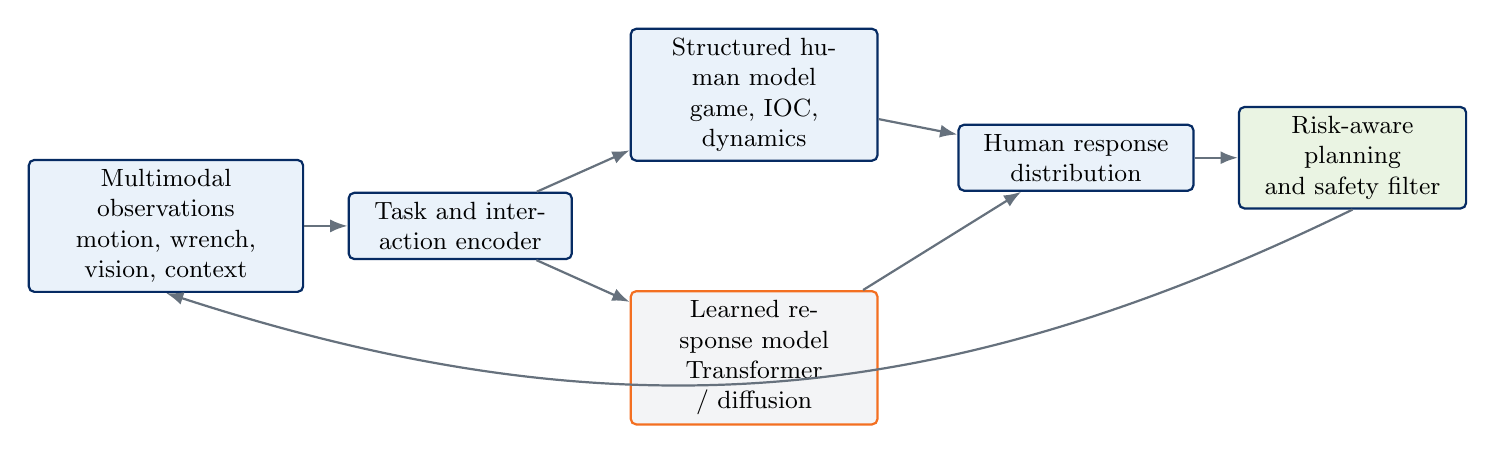
\begin{tikzpicture}[
  node distance=0.48cm and 0.55cm,
  box/.style={rounded corners=2pt,draw=navy,thick,fill=lightblue,align=center,minimum height=0.72cm,font=\small},
  learned/.style={box,draw=orange,fill=warmgray},
  control/.style={box,fill=lightgreen},
  arr/.style={-{Latex[length=2.2mm]},thick,draw=muted}
]
\node[box,text width=3.25cm] (obs) {Multimodal observations\\motion, wrench, vision, context};
\node[box,text width=2.6cm,right=of obs] (enc) {Task and interaction encoder};
\node[box,text width=2.9cm,above right=0.38cm and 0.72cm of enc] (game) {Structured human model\\game, IOC, dynamics};
\node[learned,text width=2.9cm,below right=0.38cm and 0.72cm of enc] (learn) {Learned response model\\Transformer / diffusion};
\node[box,text width=2.75cm,right=1.0cm of game,yshift=-0.8cm] (dist) {Human response distribution};
\node[control,text width=2.65cm,right=of dist] (plan) {Risk-aware planning\\and safety filter};
\draw[arr] (obs)--(enc);
\draw[arr] (enc)--(game);
\draw[arr] (enc)--(learn);
\draw[arr] (game)--(dist);
\draw[arr] (learn)--(dist);
\draw[arr] (dist)--(plan);
\draw[arr,bend left=22] (plan.south) to (obs.south);
\end{tikzpicture}
}\textcolor{pink}{the bottom arrow line covered one block encircled in orange line}
\vspace{0.3cm}
\begin{block}{Design principle}
The structured component explains behavior; the learned component captures multimodality and model mismatch; online adaptation personalizes both to the current human.
\end{block}


\end{frame}

\begin{frame}{SP1: Build the physical evidence base}
\footnotesize
\begin{columns}[T,onlytextwidth]
\column{0.49\textwidth}
\begin{block}{Theme and focus}
\textbf{Physically grounded multimodal data}
\begin{itemize}
  \item Build shared-object transport experiments
  \item Synchronize motion, object state, and force/torque
  \item Create ambiguous paths, role switching, and strategy changes
  \item Compare motion-only, wrench-only, and multimodal inference
\end{itemize}
\end{block}
\column{0.47\textwidth}
\begin{alertblock}{Challenges $\rightarrow$ solutions}
\begin{itemize}
  \item No direct intent labels $\rightarrow$ hierarchical task/strategy/action labels
  \item Noisy contact data $\rightarrow$ filtering and contact-state estimation
  \item High person variability $\rightarrow$ probabilistic latent-state models
  \item Costly data $\rightarrow$ human--human, simulation, and HRI data mixture
\end{itemize}
\end{alertblock}
\end{columns}
\vspace{0.18cm}
\paperout{A multimodal benchmark and systematic study of force/torque for human intent inference.}

\textcolor{pink}{this page is too vague. what is the reasonable human intension model Output? cost function features? desired object trajectories? Or "把 intention 表示成一个动态系统或 vector field

不估计 cost，而是假设 human 希望物体服从某个局部动力系统：

x
˙
O
	​

=f
H
	​

(x
O
	​

;θ
H
	​

)

例如一个简单的 attractor model：

p
˙
	​

O
	​

=K
p
	​

(p
H
∗
	​

−p
O
	​

)
R
˙
O
	​

=f
R
	​

(R
O
	​

,R
H
∗
	​

)

这里 human intent 就是：

θ
H
	​

=(p
H
∗
	​

,R
H
∗
	​

,K
p
	​

,K
R
	​

)

分别表示：

期望物体位置；
期望姿态；
平移和旋转的积极程度。

这样就不需要假设 human 在解一个完整 optimal control problem。robot 只要根据最近的 object motion、human wrench 和 tracking error 在线估计 DS 参数。" ?
} 
\end{frame}

\begin{frame}[shrink=6]{SP2: Make intent and preference explicit}
\footnotesize
\begin{columns}[T,onlytextwidth]
\column{0.48\textwidth}
\begin{block}{Bounded-rational human model}
\[
J_H=\sum_t {w_t^H}^{\!\top}\phi_\psi(x_t,u_t^H,u_t^R,c)
\]
Reusable features may represent progress, pose, effort, interaction force, safety, smoothness, and coordination.
\begin{itemize}
  \item Infer intent, role, preference, and rationality online
  \item Represent the human's belief about robot intent
  \item Treat the human as another adapting learner
\end{itemize}
\end{block}
\column{0.48\textwidth}
\begin{alertblock}{Challenges $\rightarrow$ solutions}
\begin{itemize}
  \item Cost identifiability $\rightarrow$ Bayesian / maximum-entropy IOC
  \item Ambiguous intent $\rightarrow$ informative robot actions
  \item Unknown adaptation $\rightarrow$ latent learning-state estimation
  \item Online computation $\rightarrow$ local game approximations and MPC
\end{itemize}
\end{alertblock}
\end{columns}
\vspace{0.15cm}
\paperout{Peer-aware intent and preference inference for physical co-manipulation.}
\end{frame}

\begin{frame}[shrink=8]{SP3: Learn responses to possible robot actions}
\footnotesize
\begin{columns}[T,onlytextwidth]
\column{0.49\textwidth}
\begin{block}{Interactive response prediction}
\[
p_\psi(u^H_{\mathrm{future}}\mid h_t,c,u^R_{\mathrm{future}})
\]
\begin{itemize}
  \item Predict multimodal human response trajectories
  \item Condition on motion, wrench, context, and candidate robot actions
  \item Predict uncertainty and latent-state transitions
  \item Compare Transformer, diffusion, and latent-variable models
\end{itemize}
\end{block}
\column{0.47\textwidth}
\begin{alertblock}{Challenges $\rightarrow$ solutions}
\begin{itemize}
  \item Limited action coverage $\rightarrow$ diverse robot probing
  \item Correlation vs. response $\rightarrow$ counterfactual conditioning
  \item OOD actions $\rightarrow$ uncertainty estimation and detection
  \item Slow inference $\rightarrow$ distilled or few-step diffusion
\end{itemize}
\end{alertblock}
\end{columns}
\vspace{0.15cm}
\paperout{Robot-action-conditioned diffusion models for multimodal human response prediction.}
\end{frame}

\begin{frame}{SP4: Close the loop through safe control}
\footnotesize
\begin{columns}[T,onlytextwidth]
\column{0.48\textwidth}
\begin{block}{Human-model-aware planning}
\[
u_R^*=\arg\min_{u_R}\;\mathbb{E}_{u_H\sim p_\psi}[J_R]
\]
subject to object dynamics, actuation, force, collision, and safety constraints.
\begin{itemize}
  \item Optimize progress, team effort, and interaction force
  \item Replan as the human model is updated
  \item Use a safety filter before execution
\end{itemize}
\end{block}
\column{0.48\textwidth}
\begin{alertblock}{Challenges $\rightarrow$ solutions}
\begin{itemize}
  \item Prediction error $\rightarrow$ short-horizon MPC
  \item Distributional complexity $\rightarrow$ scenario sampling
  \item Excess conservatism $\rightarrow$ risk-sensitive objectives
  \item Hard safety limits $\rightarrow$ CBF / constrained safety filter
\end{itemize}
\end{alertblock}
\end{columns}
\vspace{0.15cm}
\paperout{Uncertainty-aware planning and safe control with interactive human response models.}
\end{frame}

\begin{frame}[shrink=7]{SP5: Transfer human concepts across tasks and people}
\footnotesize
\begin{columns}[T,onlytextwidth]
\column{0.48\textwidth}
\begin{block}{Task-conditioned generalization}
Shared human latent concepts:
\begin{itemize}
  \item intent and local strategy;
  \item leader--follower role and compliance;
  \item effort, safety, and interaction preferences;
  \item reaction delay and adaptation state.
\end{itemize}
Encode goals, object dynamics, geometry, contacts, and constraints as task context. Adapt only latent states, preference weights, or a small adapter online.
\end{block}
\column{0.48\textwidth}
\begin{alertblock}{Challenges $\rightarrow$ solutions}
\begin{itemize}
  \item Different task structures $\rightarrow$ object-centric states and wrenches
  \item Limited physical data $\rightarrow$ simulation and human--human pretraining
  \item Negative transfer $\rightarrow$ structured task encoders
  \item Unstable personalization $\rightarrow$ Bayesian updates or small adapters
\end{itemize}
\end{alertblock}
\end{columns}
\vspace{0.15cm}
\paperout{A task-conditioned human model for cross-task co-manipulation and online personalization.}
\end{frame}

\begin{frame}[shrink=5]{Five subprojects answer one connected question chain}
\centering
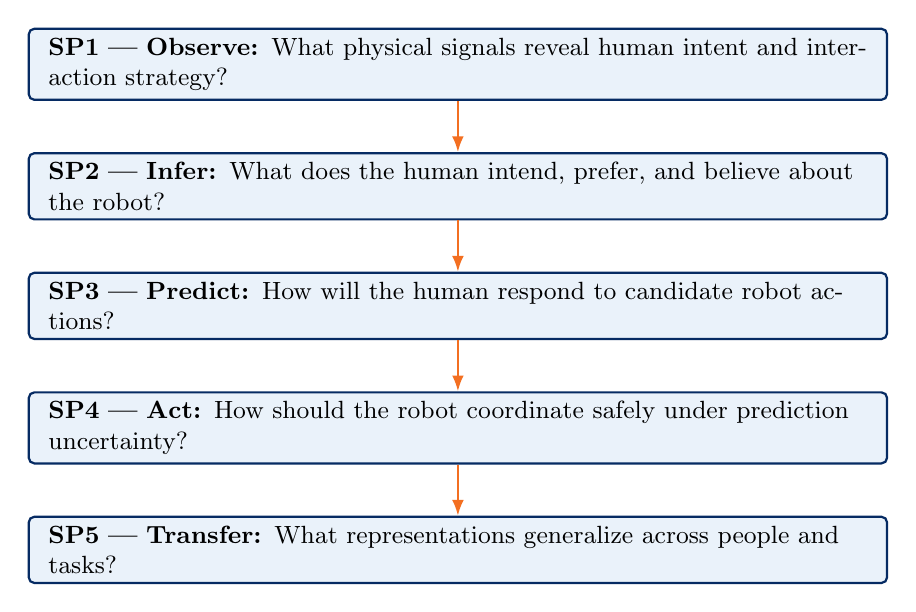
\begin{tikzpicture}[
  node distance=0.65cm,
  pbox/.style={rounded corners=2pt,draw=navy,thick,fill=lightblue,minimum width=10.9cm,minimum height=0.68cm,align=left,text width=10.4cm,font=\small},
  arr/.style={-{Latex[length=2mm]},thick,draw=orange}
]
\node[pbox] (p1) {\textbf{SP1 --- Observe:} What physical signals reveal human intent and interaction strategy?};
\node[pbox,below=of p1] (p2) {\textbf{SP2 --- Infer:} What does the human intend, prefer, and believe about the robot?};
\node[pbox,below=of p2] (p3) {\textbf{SP3 --- Predict:} How will the human respond to candidate robot actions?};
\node[pbox,below=of p3] (p4) {\textbf{SP4 --- Act:} How should the robot coordinate safely under prediction uncertainty?};
\node[pbox,below=of p4] (p5) {\textbf{SP5 --- Transfer:} What representations generalize across people and tasks?};
\draw[arr] (p1)--(p2); \draw[arr] (p2)--(p3); \draw[arr] (p3)--(p4); \draw[arr] (p4)--(p5);
\end{tikzpicture}
\end{frame}

\begin{frame}[shrink=6]{A focused transport study can test the core hypothesis}
\begin{columns}[T,onlytextwidth]
\column{0.47\textwidth}
\begin{block}{Initial task}
A human and robot transport a shared object through an environment with multiple feasible paths.
\end{block}
\textbf{Model inputs}
\begin{itemize}
  \item Object and human motion
  \item Interaction force/torque
  \item Goal and environment geometry
  \item Candidate robot actions
\end{itemize}
\column{0.49\textwidth}
\textbf{Comparisons}
\begin{enumerate}
  \item Reactive control without a human model
  \item Passive prediction from interaction history
  \item Structured intent inference
  \item Robot-action-conditioned prediction
  \item Hybrid structured + learned model
\end{enumerate}
\textbf{Evaluation}
\begin{itemize}
  \item Prediction accuracy and calibration
  \item Success, time, and team effort
  \item Interaction force and disagreement
  \item Adaptation, safety, and comfort violations
\end{itemize}
\end{columns}
\end{frame}

\begin{frame}[shrink=5]{The program connects human understanding to robot action}
\begin{columns}[T,onlytextwidth]
\column{0.57\textwidth}
\begin{enumerate}
  \item A physically grounded multimodal benchmark
  \item Bounded-rational, peer-aware intent inference
  \item Interactive prediction of responses to robot actions
  \item Safe planning over human response distributions
  \item Cross-task generalization and online personalization
\end{enumerate}
\column{0.39\textwidth}
\begin{alertblock}{Long-term vision}
A versatile human model that connects physical interaction, human adaptation, and robot decision-making across co-manipulation scenarios.
\end{alertblock}
\end{columns}
\vspace{0.35cm}
\begin{block}{Proposed starting point}
Use a physical collaborative-transport task to test whether force/torque sensing and robot-action-conditioned prediction improve intent inference, coordination, and safe control.
\end{block}
\end{frame}

\begin{frame}{Questions to refine the research direction}
\begin{itemize}
  \item Which physical co-manipulation task is the most useful initial test case?
  \item What sensing and robotic platforms are currently available?
  \item Should the first contribution emphasize human intent inference, interactive response prediction, or planning and control?
  \item Which components of RISE Lab's existing game-theoretic framework can be extended directly to physical coupling?
  \item What level of cross-task generalization would be most valuable for the current project?
\end{itemize}
\vspace{0.35cm}
\begin{alertblock}{Discussion objective}
Identify a focused first study that contributes to the larger goal of a generalizable and interactive human model.
\end{alertblock}
\end{frame}

\end{document}
